\chapter{系统总体设计}

本章从总体架构、功能模块、业务流程、数据结构和部署结构五个方面说明 CulCloud 的系统设计。设计目标不是简单堆叠页面功能，而是让用户端文件处理、后端任务状态、对象存储、运行日志和管理端分析形成一致的数据闭环。系统采用 React 前端、FastAPI 业务服务、MinIO 对象存储、Redis 状态与日志、Gotenberg 转换服务以及 Flask/Spark 分析服务的组合结构，使文件上传、预览、转换、PDF 页面整理和管理端观察能够在同一平台内协同运行。

\section{总体架构设计}

CulCloud 按照表示层、业务接口层、领域服务层、基础数据层和分析应用层进行分层。表示层包含用户端与管理端两类界面，用户端负责文件上传、目录整理、预览、格式转换和 PDF 编辑，管理端负责任务、日志、健康状态和分析结果观察。业务接口层由 FastAPI 提供统一入口，按文件、目录、预览、转换、任务、日志和系统健康拆分路由。领域服务层封装对象存储、文档转换、任务追踪、日志采集和健康检查。基础数据层由 MinIO、Redis 和 Gotenberg 构成，分别承担对象保存、状态保存和文档渲染转换。历史分析层由 Spark 输出聚合 JSON，Flask Analytics 提供读取接口，再由管理端 ECharts 呈现。

图 \ref{fig:chap04-layer-architecture} 给出了系统分层架构。该图强调两类数据口径：第一类是 FastAPI 直接聚合的实时运行数据，来自文件、任务、日志和系统健康接口；第二类是 Spark 处理后的历史分析样本，用于展示较长时间窗口下的文件类型、转换趋势和质量指标。二者在管理端同时出现，但语义上保持分离，避免将离线样本误认为实时业务总量。

\begin{figure}[H]
  \centering
  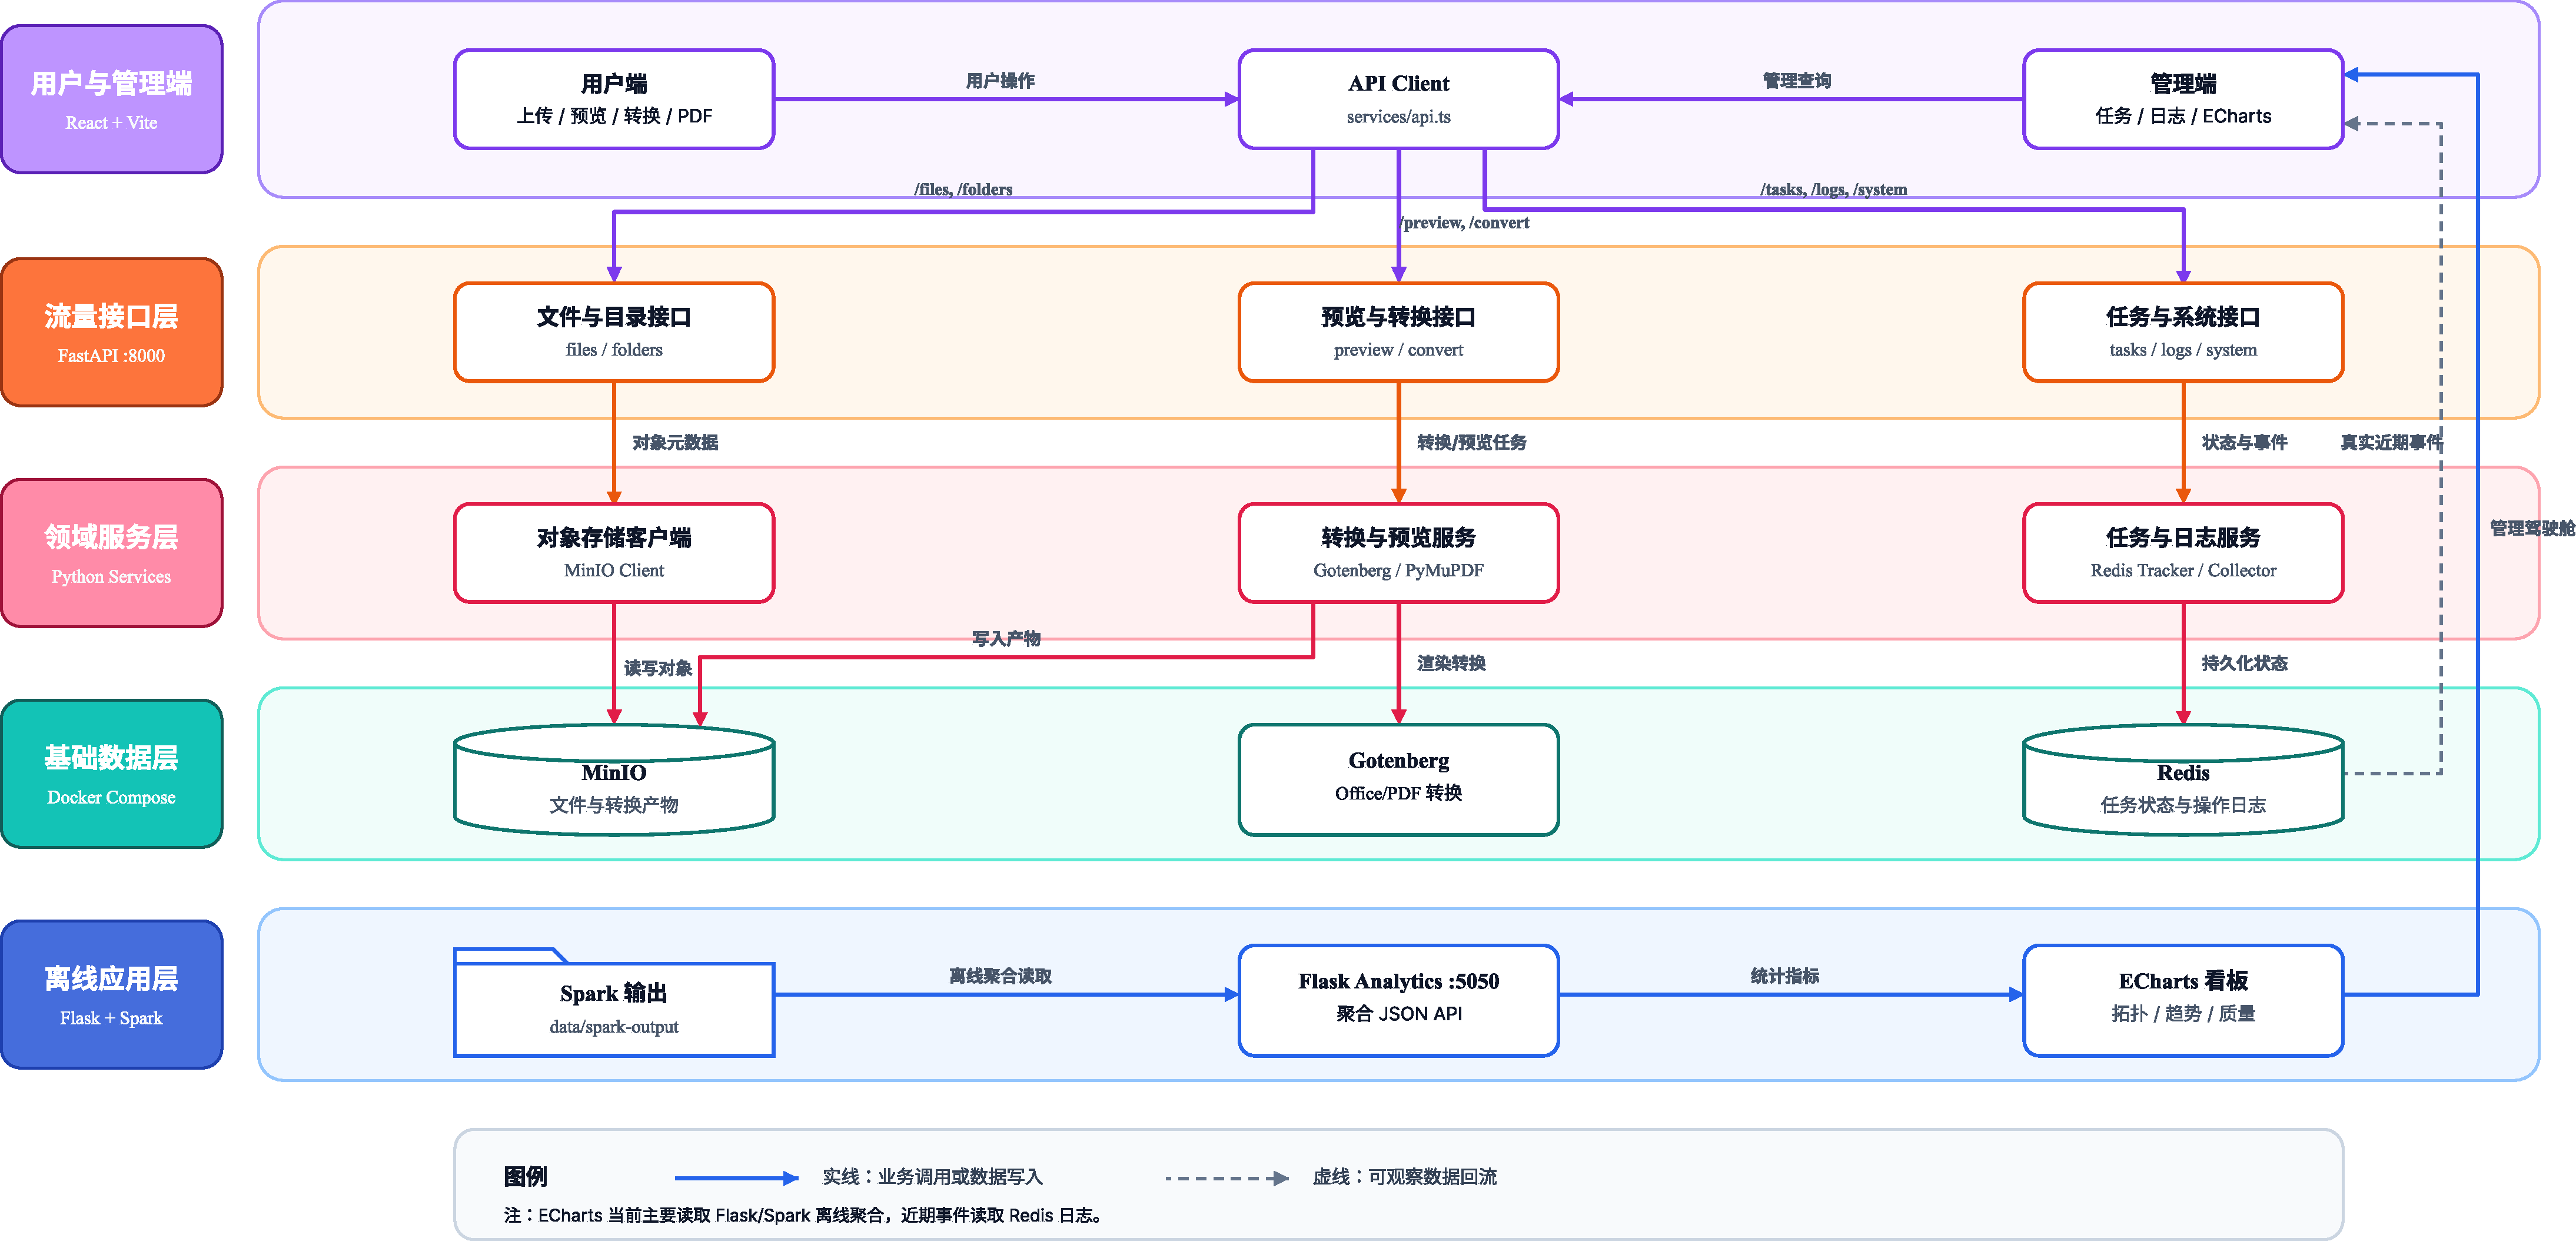
\includegraphics[width=0.96\textwidth,height=0.62\textheight,keepaspectratio]{figures-pdf/fig08-云端资料处理平台系统分层架构图.pdf}
  \caption{云端资料处理平台系统分层架构图}
  \label{fig:chap04-layer-architecture}
\end{figure}

\section{系统功能设计}

\subsection{功能模块划分}

系统围绕用户端和管理端两条主线划分为六个核心模块。用户端包含个人首页、我的文件、转换中心和 PDF 编辑室；管理端包含管理驾驶舱、任务监控和系统状态。各模块并非孤立页面，而是通过统一 API 客户端访问后端接口，再由后端服务读写 MinIO 与 Redis。表 \ref{tab:function-modules} 列出了模块边界与数据来源。

\begin{table}[H]
  \centering
  \caption{系统功能模块划分}
  \label{tab:function-modules}
  \begin{tabularx}{\textwidth}{llXX}
    \toprule
    端侧 & 模块 & 主要功能 & 数据来源 \\
    \midrule
    用户端 & 个人首页 & 文件数量、空间占用、近期任务和失败提示 & 文件接口、任务接口 \\
    用户端 & 我的文件 & 上传、目录、搜索、移动、删除和下载 & MinIO 对象元数据 \\
    用户端 & 文件预览 & PDF、图片、文本、Markdown、CSV、Office、音视频预览 & 预览接口、转换缓存 \\
    用户端 & 转换中心 & P0 白名单格式转换、任务轮询、结果下载 & 转换接口、Redis 任务状态 \\
    用户端 & PDF 编辑室 & 页面提取、排序、旋转、删除、批注和导出 & PDF 处理接口、MinIO 产物 \\
    管理端 & 管理驾驶舱 & 实时运行状态、历史分析样本和图表展示 & FastAPI、Flask/Spark、ECharts \\
    \bottomrule
  \end{tabularx}
\end{table}

图 \ref{fig:chap04-module-dependency} 展示了模块依赖关系。前端不直接访问 MinIO、Redis 或 Gotenberg，而是通过 API 客户端进入 FastAPI 路由，由路由层调用领域服务完成对象读写、转换执行和状态记录。这种设计将浏览器侧交互与基础设施细节隔离，降低了前端暴露存储地址或内部任务键的风险。

\begin{figure}[H]
  \centering
  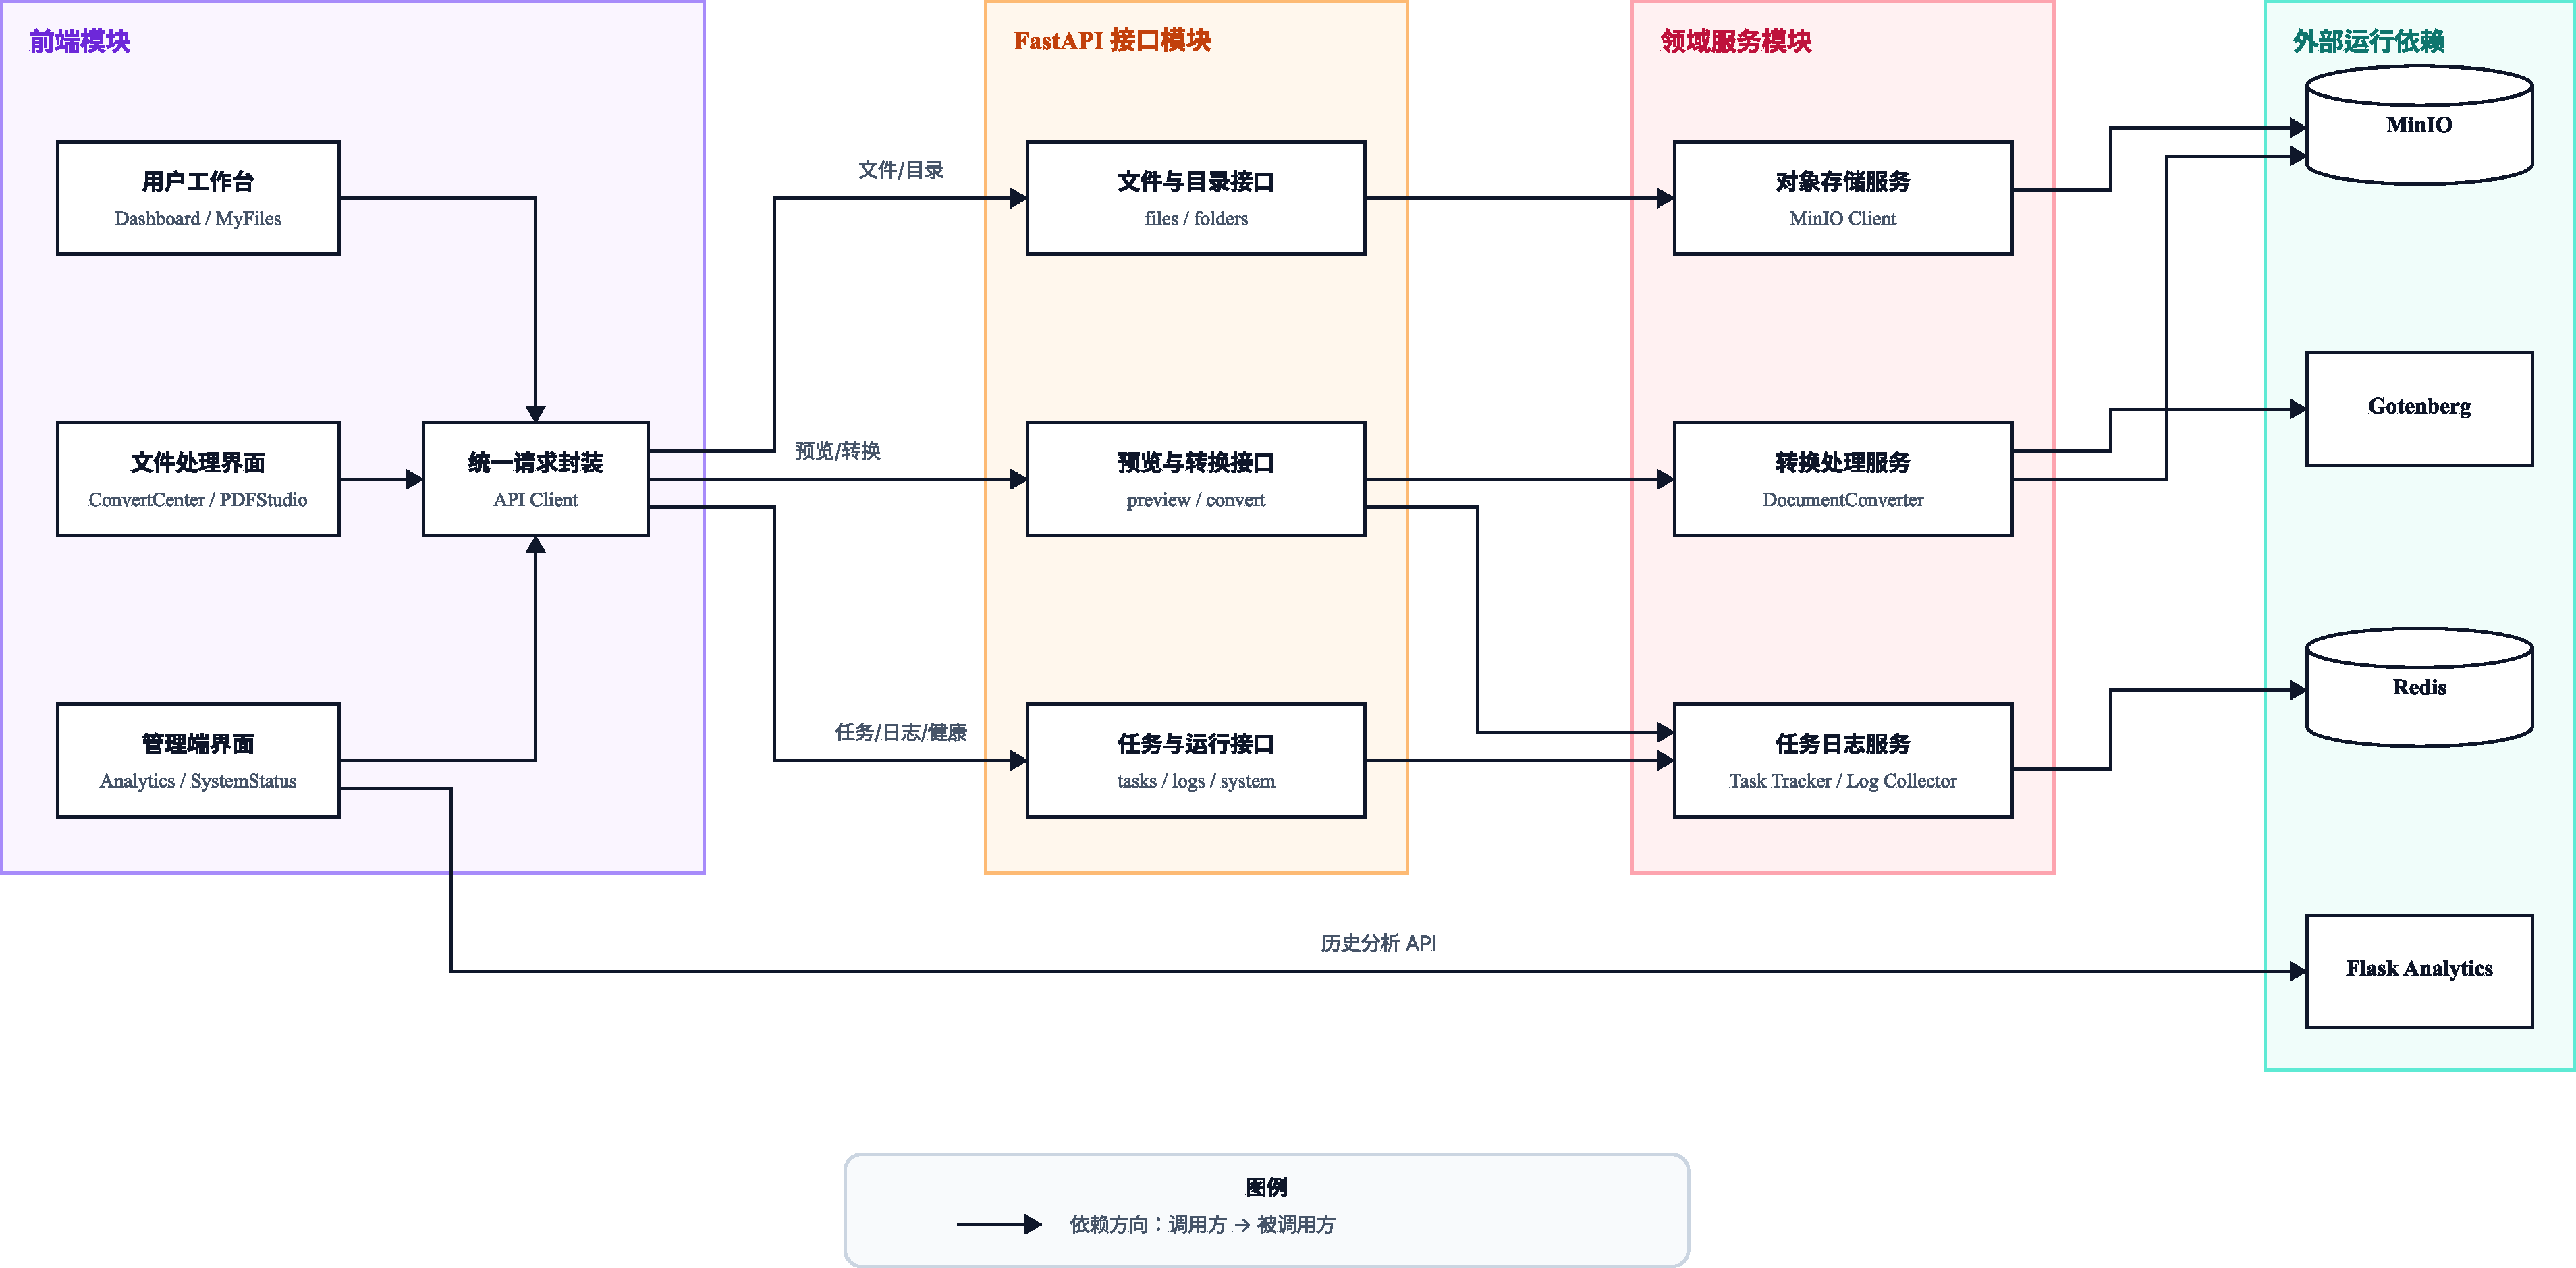
\includegraphics[width=0.96\textwidth,height=0.52\textheight,keepaspectratio]{figures-pdf/fig09-moudules-diagrams.pdf}
  \caption{前后端核心模块依赖图}
  \label{fig:chap04-module-dependency}
\end{figure}

\subsection{用户端模块}

用户端的设计重点是让普通用户以云盘方式组织资料，并在同一界面路径中完成处理。我的文件模块负责对象列表、目录前缀、类型筛选和预览入口；转换中心负责从本地或云端选择文件，按白名单提交格式转换任务；PDF 编辑室负责将 PDF 页面转为可操作页面集合，再提交页面顺序、旋转角度和批注配置生成新文件。用户端所有可生成产物的操作都应写入任务状态和事件日志，以便后续查询与管理端观察。

\subsection{管理端模块}

管理端的设计重点是观察系统运行，而不是重复用户端操作。第一屏读取 FastAPI 的文件、任务、日志和健康接口，显示当前业务系统真实状态；第二屏和第三屏读取 Spark 历史分析样本，展示文件类型分布、历史转换任务、遥测质量、存储水位和错误热力图。任务监控用于查看任务列表、队列长度和失败原因；系统状态用于观察 Redis、MinIO、Gotenberg、API 和分析服务的健康状态。

\section{业务流程设计}

系统核心业务并不是单个页面动作，而是“用户操作、后端处理、对象产物、任务状态、管理观察”的闭环。用户端上传、预览、转换和 PDF 导出会进入 FastAPI 路由，后端根据任务类型读写 MinIO 对象，并将任务状态与事件日志写入 Redis；管理端第一屏再从文件、任务、日志和健康接口读取实时数据。图 \ref{fig:chap04-business-loop} 展示了这一业务闭环，它用于说明用户端业务增量为什么能够实时反映到管理端运行指标中。

\begin{figure}[H]
  \centering
  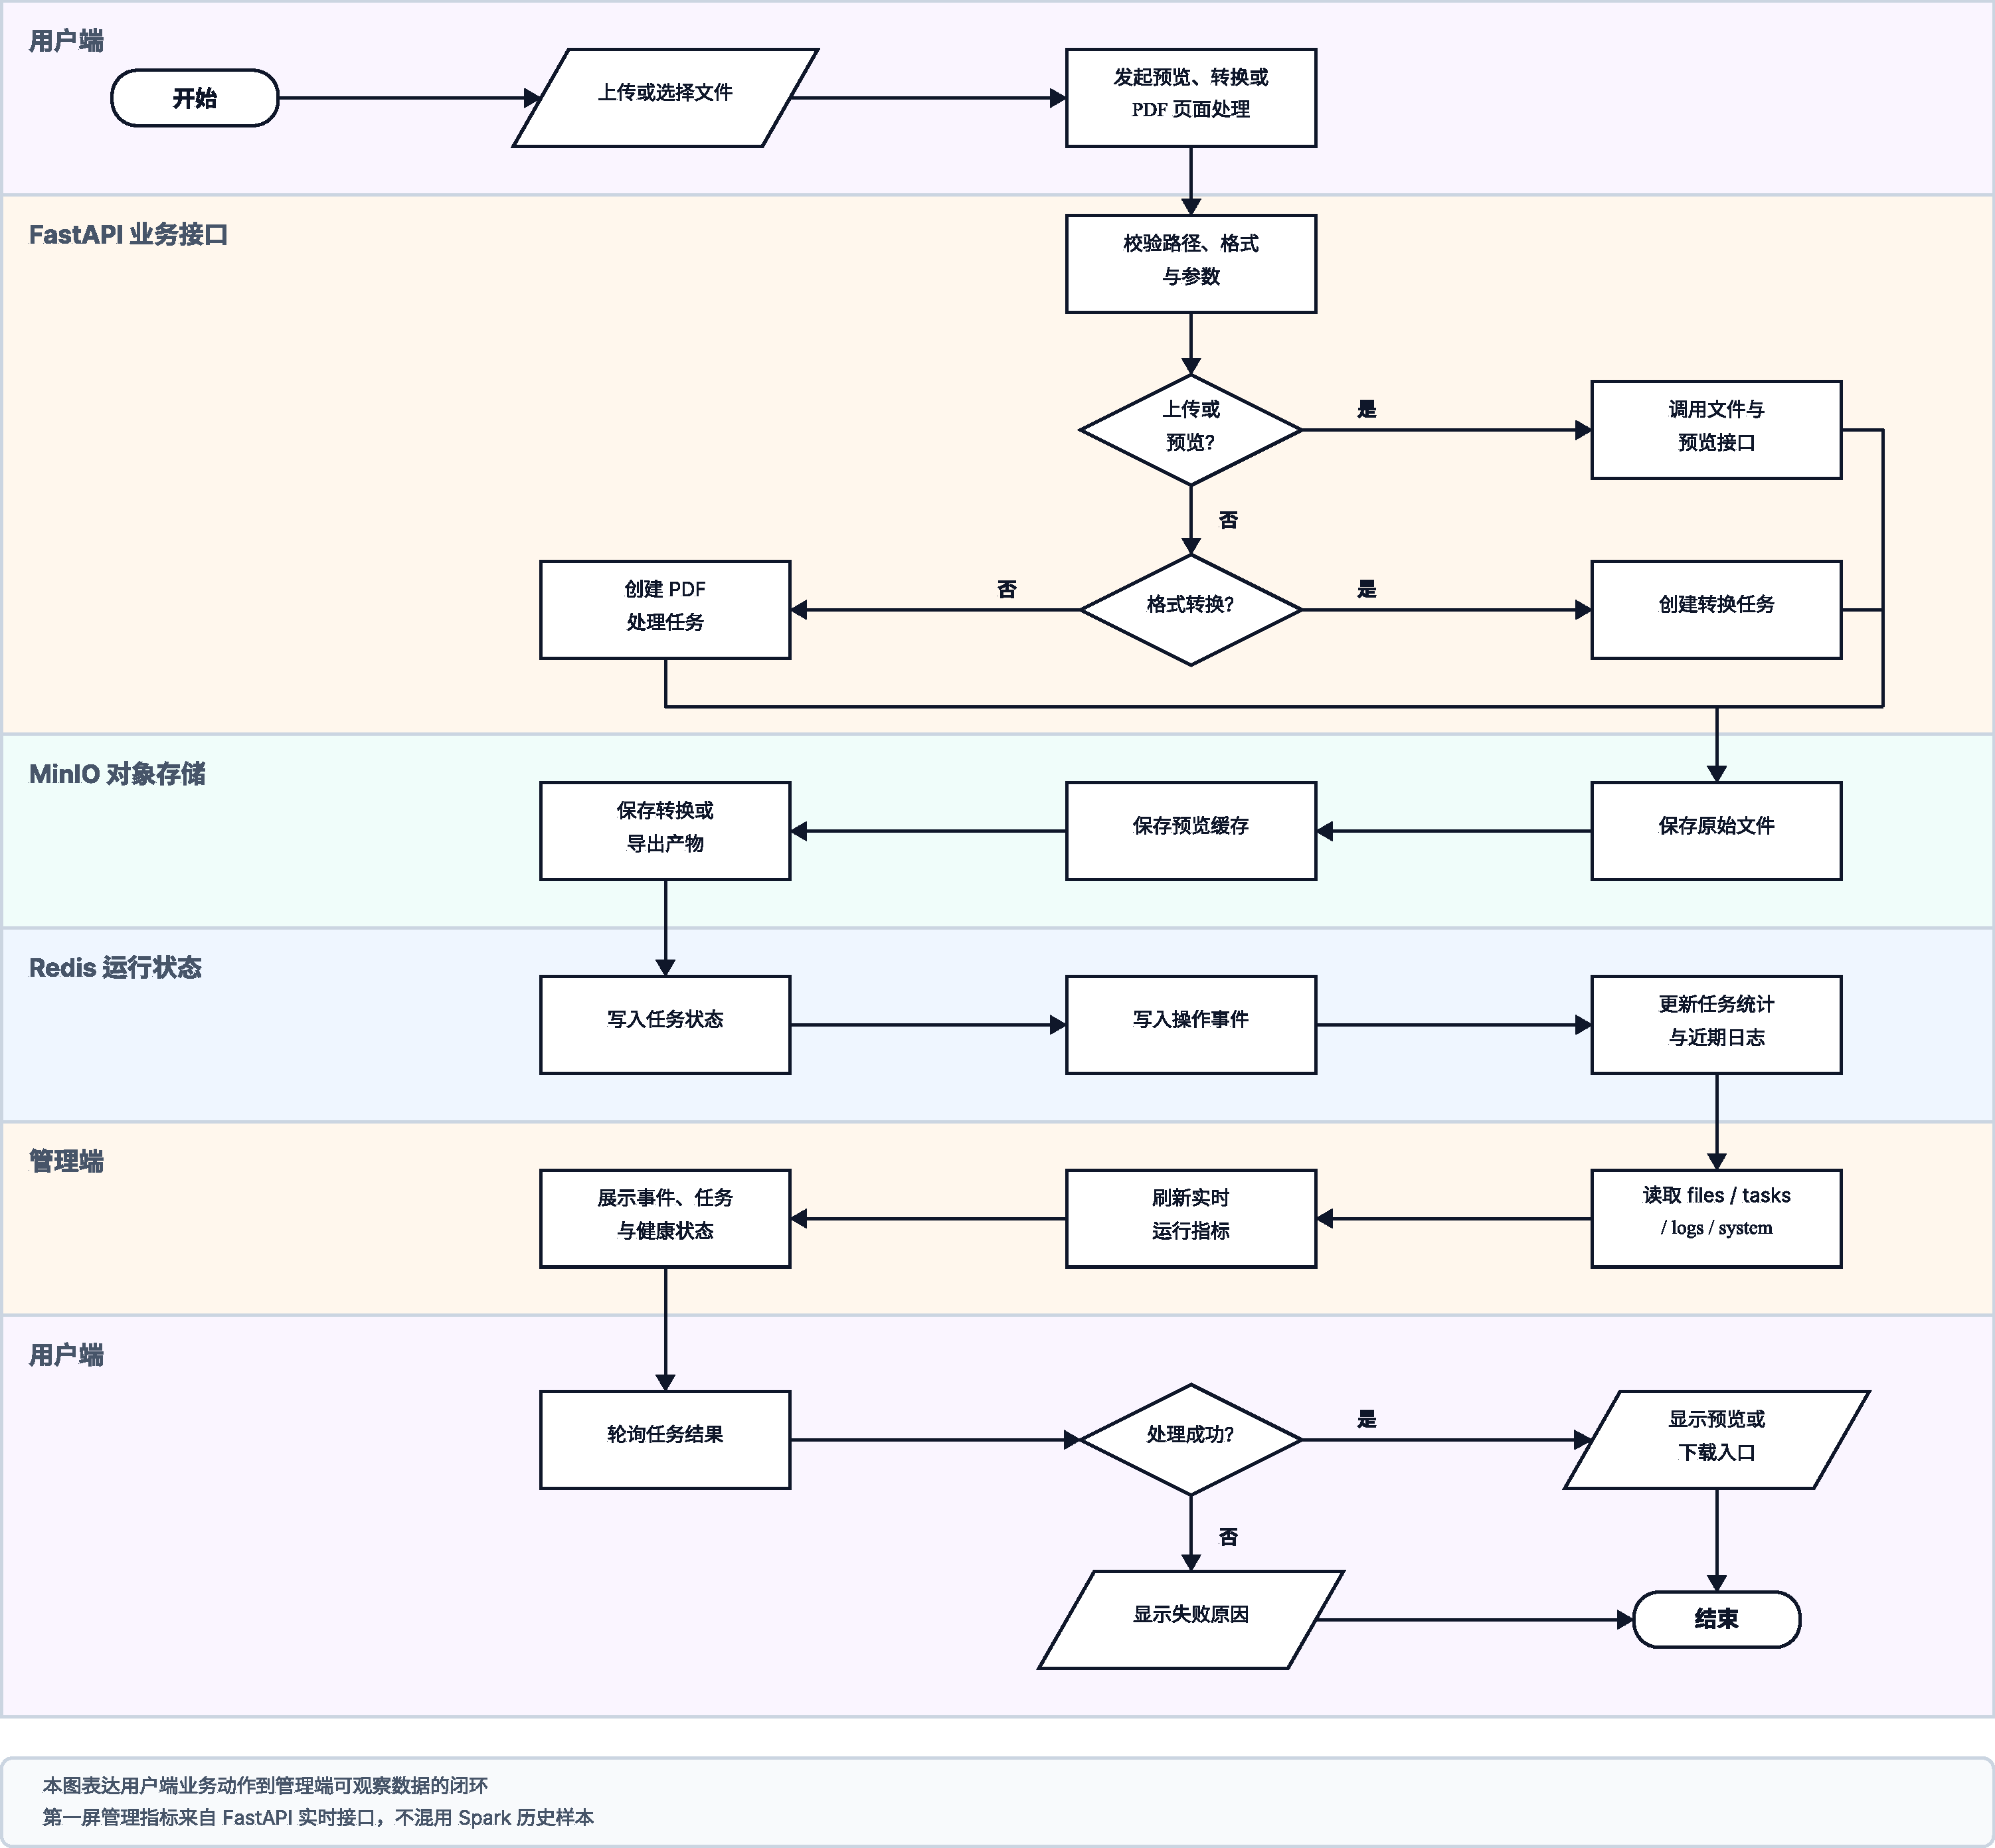
\includegraphics[width=0.96\textwidth,height=0.58\textheight,keepaspectratio]{figures-pdf/fig16-核心业务闭环流程图.pdf}
  \caption{核心业务闭环流程图}
  \label{fig:chap04-business-loop}
\end{figure}

\subsection{文件上传与预览流程}

文件上传流程从用户选择文件开始。前端携带当前目录前缀和相对路径调用上传接口，后端校验路径合法性后生成对象名称，将文件写入 MinIO，并记录上传事件。列表刷新时，后端根据对象名前缀和 \texttt{.keep} 空对象合成文件夹与文件视图。预览流程则由文件类型决定：图片、PDF、音频和视频可直接返回内容地址；TXT、Markdown 和 CSV 由后端生成可读内容；Office 文件优先生成 PDF 预览缓存。图 \ref{fig:chap04-preview-flow} 用活动图表示了上传、列表刷新和预览之间的责任边界。

\begin{figure}[H]
  \centering
  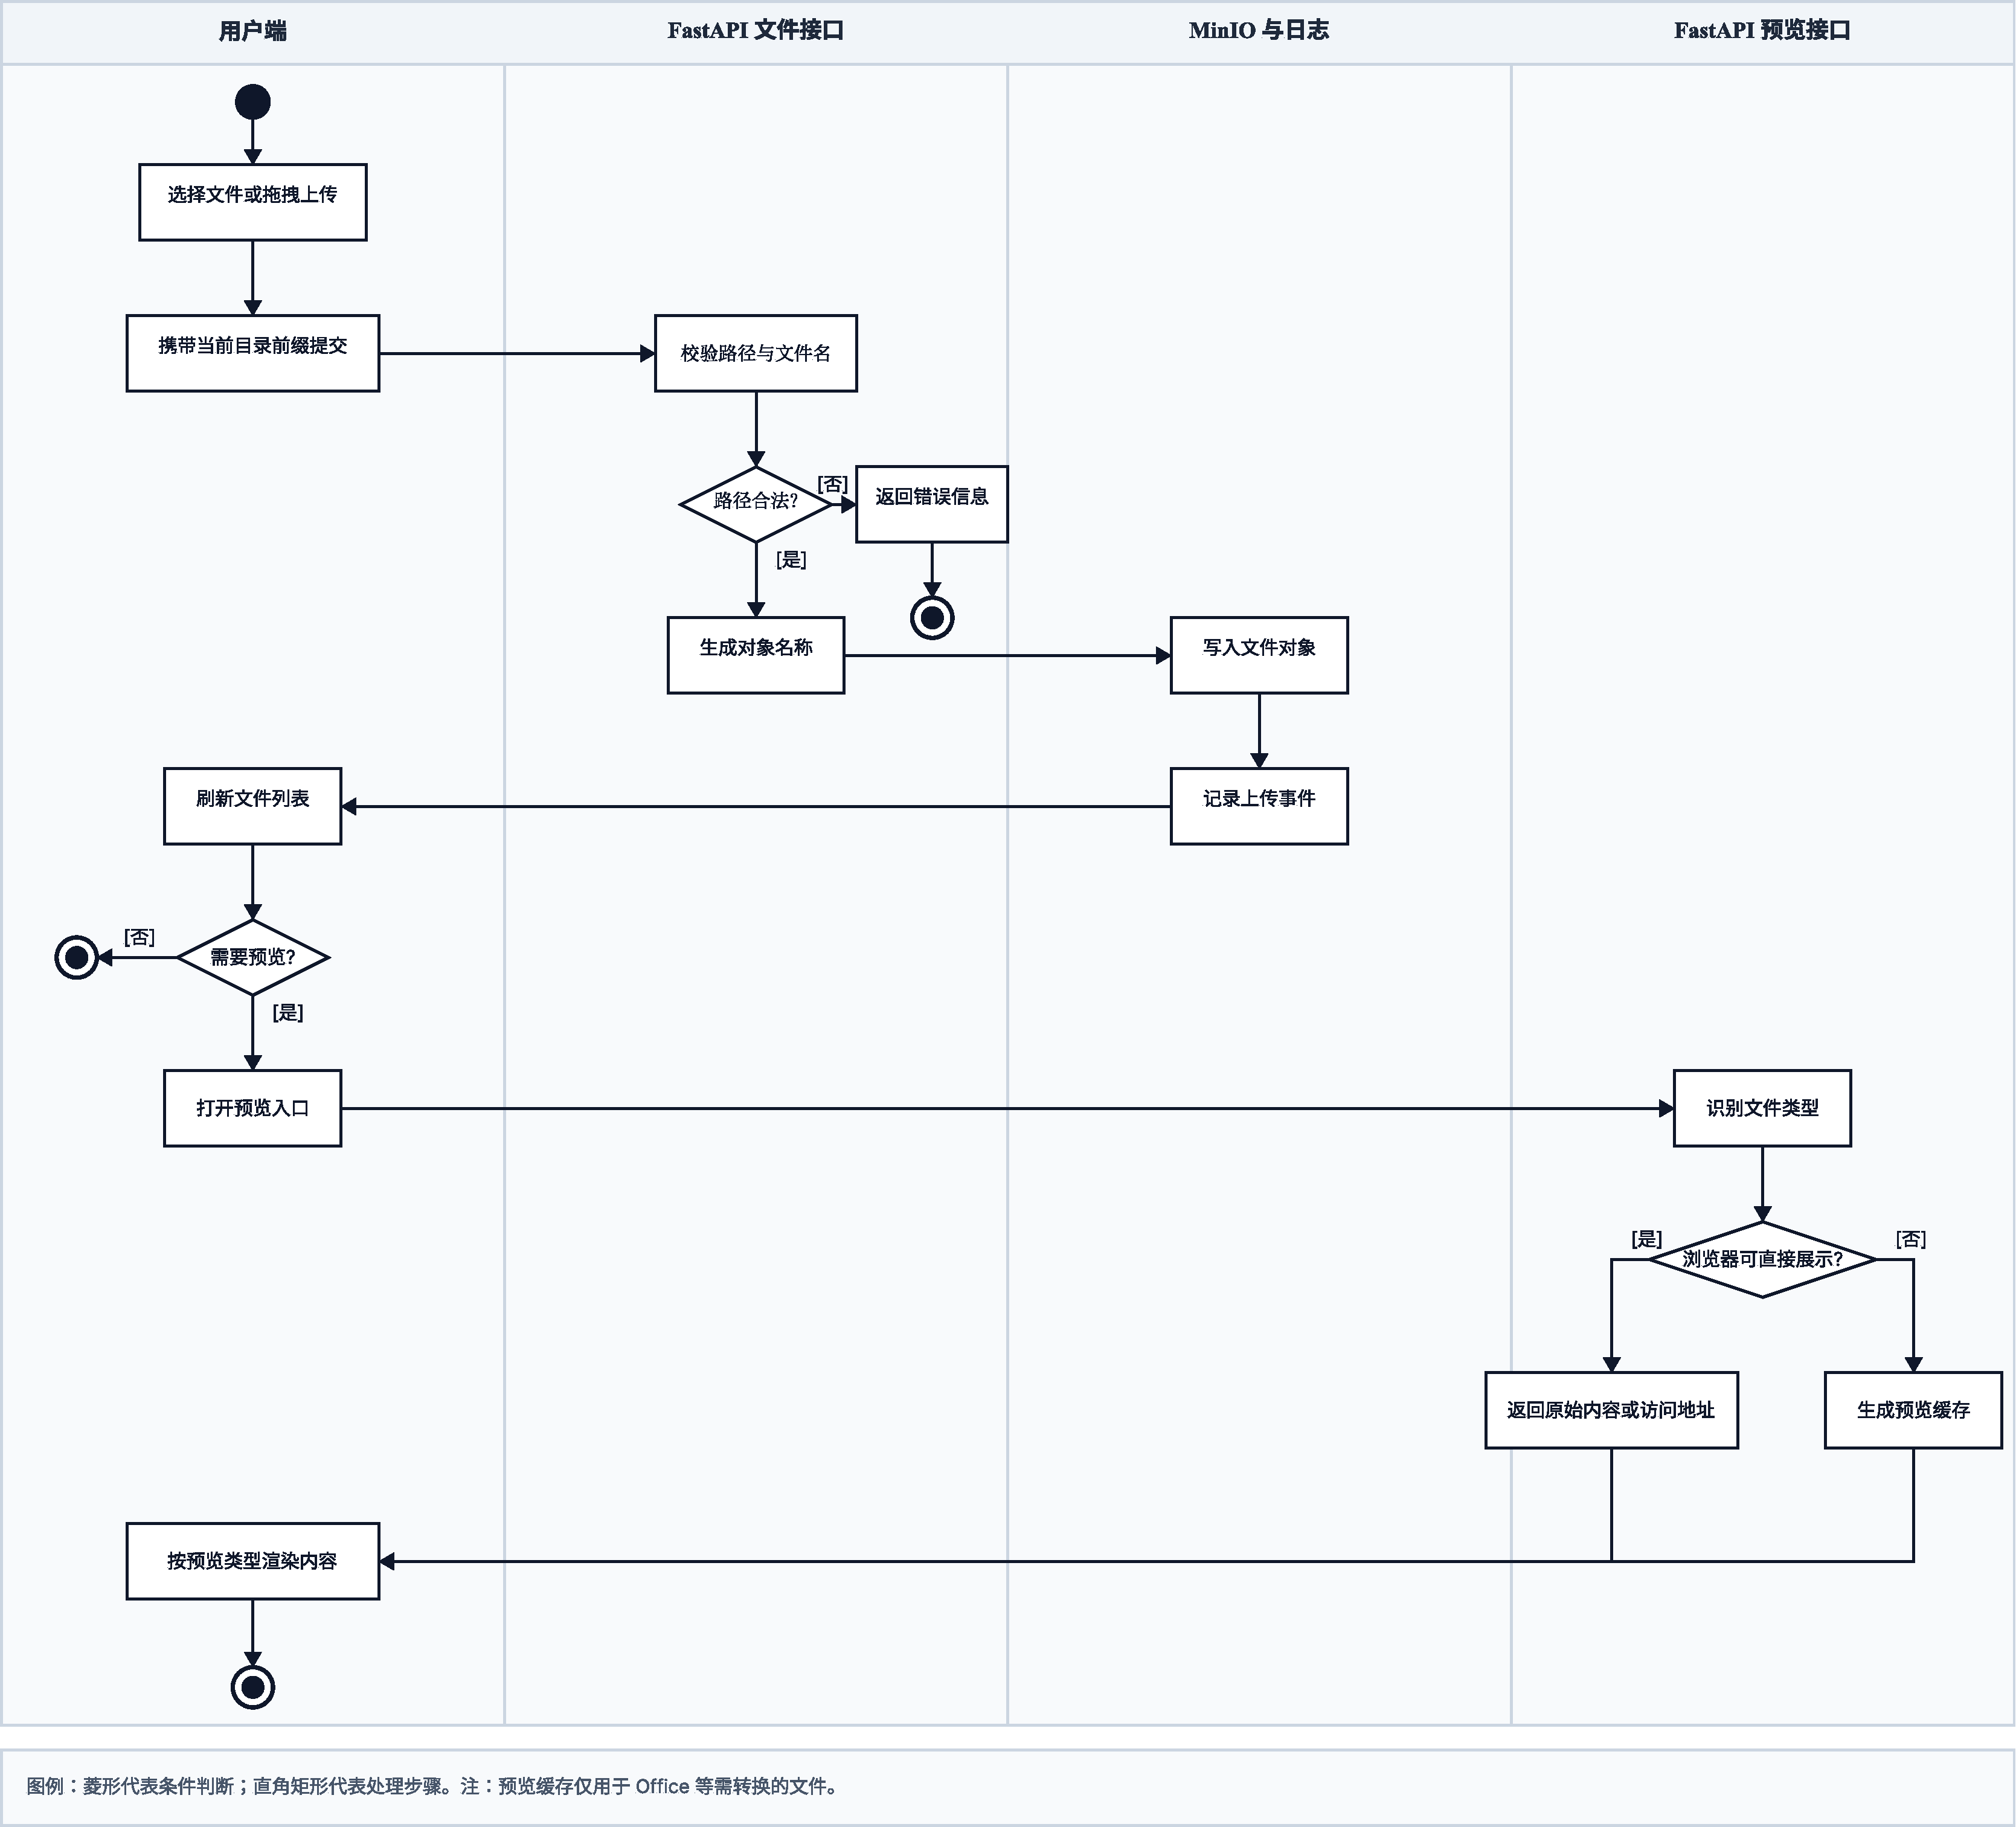
\includegraphics[width=0.92\textwidth,height=0.58\textheight,keepaspectratio]{figures-pdf/fig10-文件预览活动图.pdf}
  \caption{文件上传、整理与预览活动图}
  \label{fig:chap04-preview-flow}
\end{figure}

\subsection{格式转换流程}

格式转换采用“提交任务、后台处理、短轮询读取状态”的异步流程。用户在转换中心选择目标格式后，前端调用转换接口；后端首先执行 P0 白名单校验，通过后创建任务标识并写入 Redis，随后使用 FastAPI BackgroundTasks 启动后台转换逻辑。转换任务进入处理中状态后，从 MinIO 读取源文件，调用 Gotenberg 或本地转换库生成结果，最终将产物写回 \texttt{conversions/} 前缀并更新任务状态。前端通过任务查询接口读取状态、错误信息和结果地址。图 \ref{fig:chap04-conversion-sequence} 展示了该时序。

该流程的设计重点有三点。第一，转换能力必须先经过白名单过滤，防止页面上未开放的实验能力被直接提交到后端执行。第二，转换结果统一通过后端文件内容接口代理下载，而不是把对象存储内部地址直接暴露给浏览器。第三，任务状态与日志事件同步写入，使“转换完成”“转换失败”“结果可下载”三个判断来自同一后端事实，而不是分别由前端按钮状态推断。

\begin{figure}[H]
  \centering
  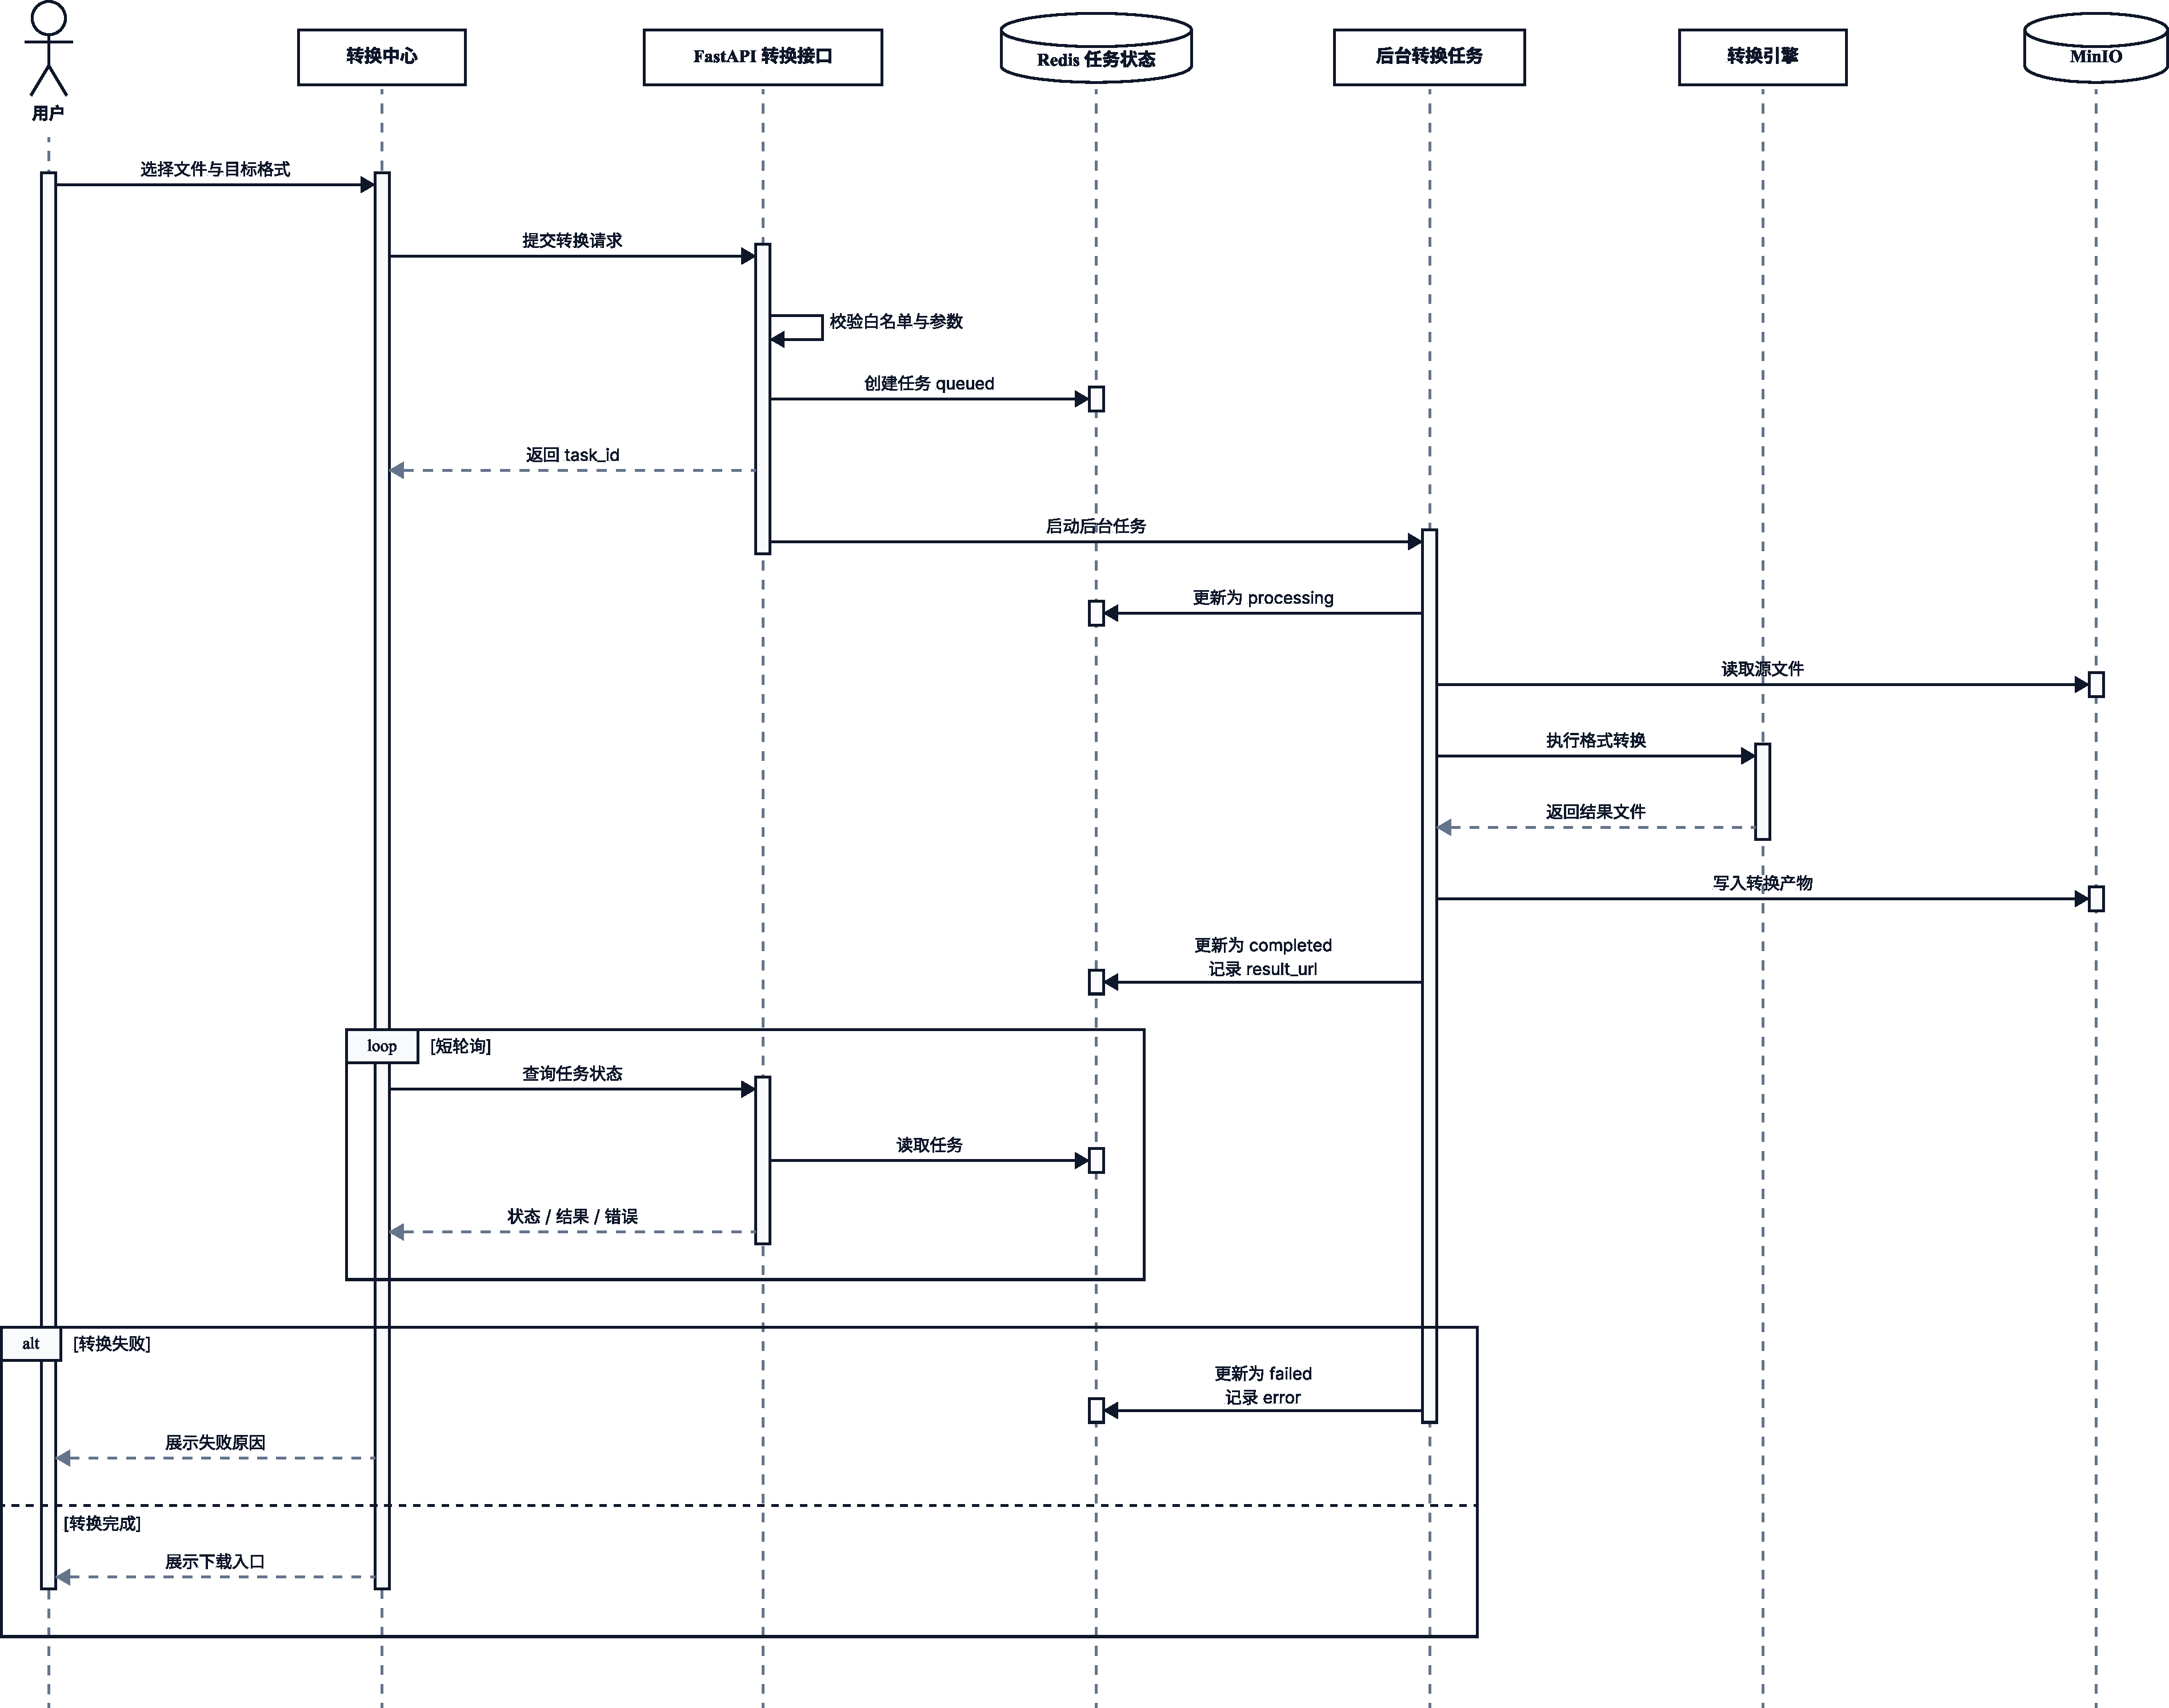
\includegraphics[width=0.96\textwidth,height=0.55\textheight,keepaspectratio]{figures-pdf/fig11-格式转换任务时序图.pdf}
  \caption{格式转换任务时序图}
  \label{fig:chap04-conversion-sequence}
\end{figure}

\subsection{PDF 编辑与导出流程}

PDF 编辑室将原始 PDF 拆解为页面图像，并在前端维护页面顺序、旋转角度、删除状态和批注对象。用户提交导出时，前端把页面配置传给 \texttt{/api/v1/convert/pdf/process}，后端根据配置重新组装 PDF 页面并写入批注，生成的新文件保存到 MinIO。该流程的关键设计是将“页面操作状态”与“最终 PDF 产物”分离：前端负责交互和坐标记录，后端负责文件级重组与输出。图 \ref{fig:chap04-pdf-flow} 展示了 PDF 编辑与导出流程。

\begin{figure}[H]
  \centering
  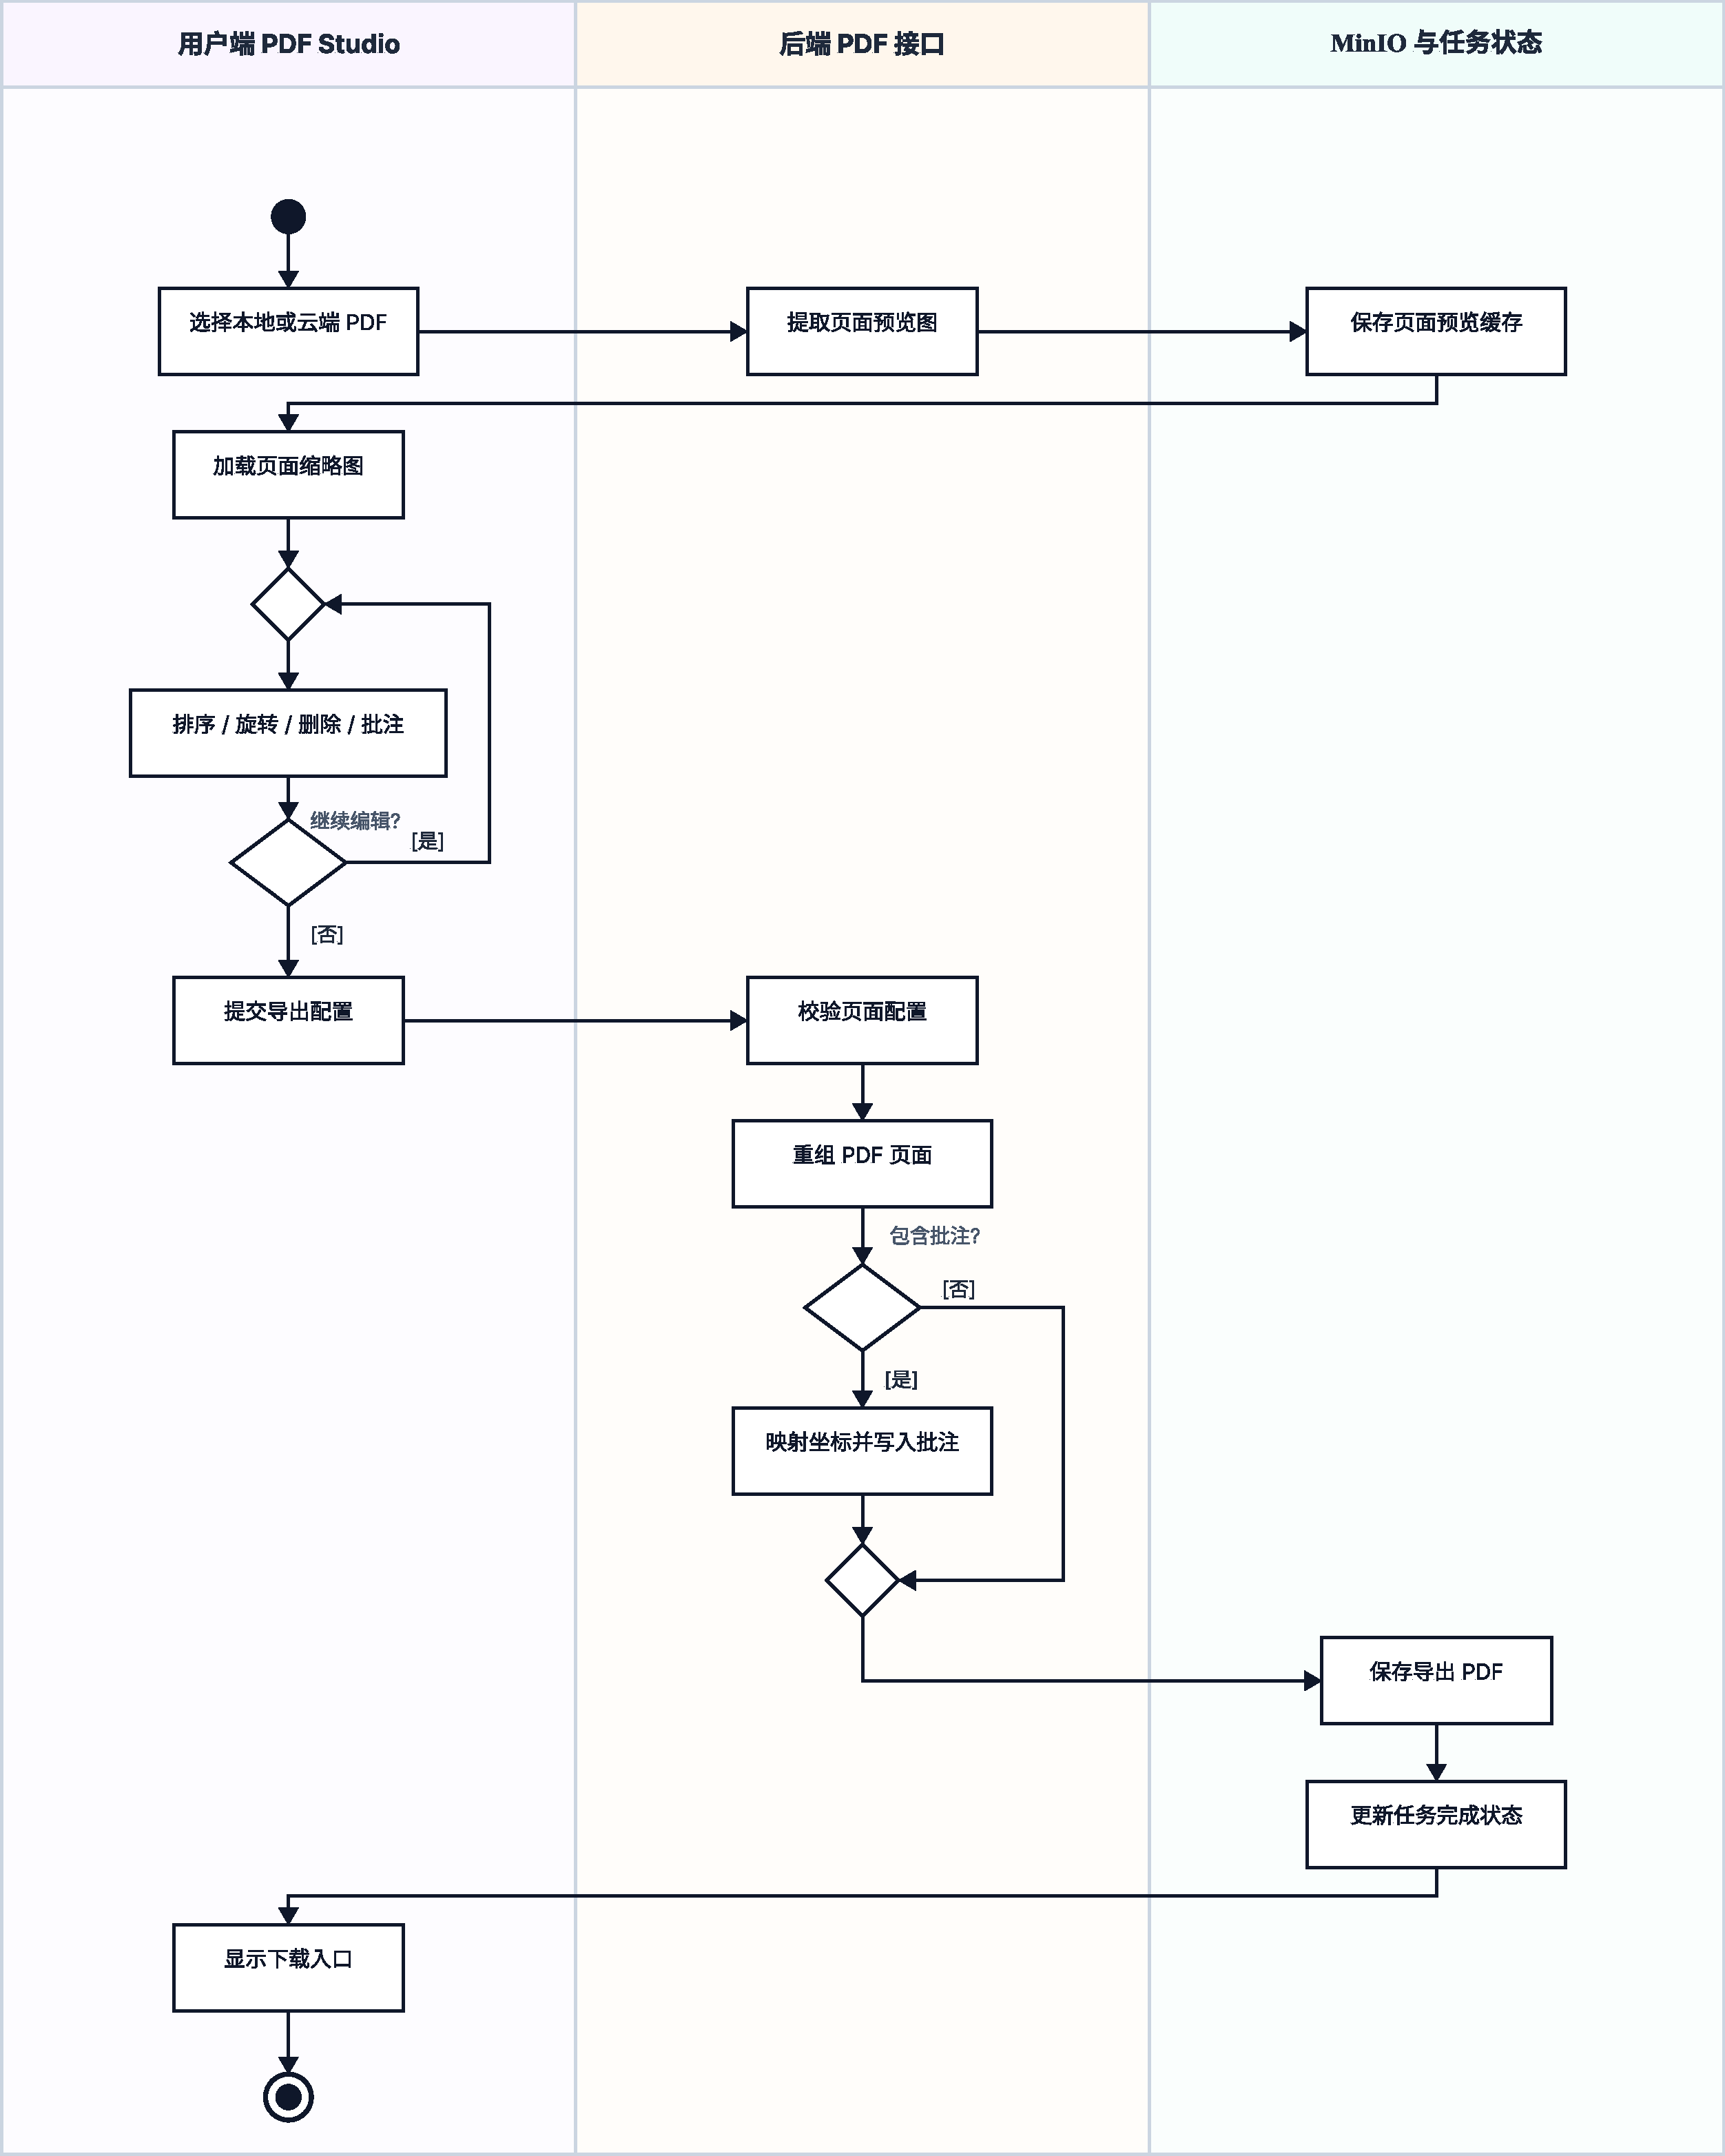
\includegraphics[width=0.90\textwidth,height=0.55\textheight,keepaspectratio]{figures-pdf/fig12-pdf编辑和批注导出活动图.pdf}
  \caption{PDF 编辑室页面整理与导出活动图}
  \label{fig:chap04-pdf-flow}
\end{figure}

\section{核心算法设计}

\subsection{预览类型分派算法}

文件预览需要在多种格式之间做稳定分派。设计上，前端不直接解析所有文件，而是由后端根据对象名和扩展名返回预览类型、内容地址和可预览状态。算法 \ref{alg:preview-dispatch} 给出了预览分派规则。该算法把二进制直读、文本结构化渲染、Office 预览缓存和不可预览状态区分开，便于第 5 章在 \texttt{preview.py} 与 \texttt{services/preview.py} 中落地。

\begin{algorithm}[H]
  \caption{文件预览类型分派算法}
  \label{alg:preview-dispatch}
  \renewcommand{\algorithmicrequire}{\textbf{输入：}}
  \renewcommand{\algorithmicensure}{\textbf{输出：}}
  \begin{algorithmic}[1]
    \Require 文件对象名 $objectName$，文件扩展名 $ext$
    \Ensure 预览类型 $previewType$ 与内容地址 $contentUrl$
    \If{$ext$ 属于 PDF、图片、音频或视频}
      \State 返回后端内容代理地址
    \ElsIf{$ext$ 属于 TXT、Markdown 或 CSV}
      \State 读取对象内容并生成结构化响应
    \ElsIf{$ext$ 属于 Office 文档}
      \State 查询或生成 PDF 预览缓存
    \Else
      \State 返回不可预览状态和下载入口
    \EndIf
  \end{algorithmic}
\end{algorithm}

\subsection{异步任务状态算法}

格式转换和 PDF 导出均属于耗时文件处理任务。系统采用“先建任务、后处理文件、再更新终态”的设计，避免用户请求长时间阻塞。算法 \ref{alg:async-task-process} 给出了异步处理的统一状态更新规则。任务必须经历等待、处理中、成功或失败状态，成功路径需要写入对象产物和结果地址，失败路径需要写入错误原因。

\begin{algorithm}[H]
  \caption{异步文件处理任务状态更新算法}
  \label{alg:async-task-process}
  \renewcommand{\algorithmicrequire}{\textbf{输入：}}
  \renewcommand{\algorithmicensure}{\textbf{输出：}}
  \begin{algorithmic}[1]
    \Require 任务编号 $taskId$，输入文件 $file$，处理类型 $kind$
    \Ensure 任务终态、结果地址或错误信息
    \State 写入任务状态 $pending$
    \State 后台任务启动，写入任务状态 $processing$
    \State 记录开始事件到运行日志
    \If{$kind$ 为格式转换}
      \State 按白名单选择转换方法并生成结果字节
    \Else
      \State 按页面配置重组 PDF 页面与批注
    \EndIf
    \If{处理成功}
      \State 将结果写入 MinIO 的 \texttt{conversions/} 前缀
      \State 写入任务状态 $success$ 与 API 代理结果地址
      \State 记录完成事件到运行日志
    \Else
      \State 写入任务状态 $failed$ 与错误原因
      \State 记录失败事件到运行日志
    \EndIf
  \end{algorithmic}
\end{algorithm}

前端轮询以任务终态作为停止边界。设第 $k$ 次查询到的任务状态为 $s_k$，终态集合为 $\Omega=\{success,failed\}$，则轮询停止条件为：
\begin{equation}
  s_k \in \Omega.
  \label{eq:polling-stop}
\end{equation}
式 \ref{eq:polling-stop} 可避免任务已完成后仍持续请求后端。

\subsection{PDF 页面导出算法}

PDF 编辑室的导出需要把前端页面顺序、旋转角度、删除状态和批注对象转化为后端可写入的 PDF 产物。批注导出的关键是坐标映射。设前端画布坐标为 $(x_c,y_c)$，画布宽高为 $W_c,H_c$，PDF 页面宽高为 $W_p,H_p$，则写回 PDF 时的坐标可表示为：
\begin{equation}
  x_p=x_c\cdot\frac{W_p}{W_c},\qquad
  y_p=y_c\cdot\frac{H_p}{H_c}.
  \label{eq:pdf-coordinate-map}
\end{equation}
式 \ref{eq:pdf-coordinate-map} 说明批注位置应由画布尺寸与 PDF 页面尺寸之间的比例确定，而不是依赖浏览器缩放值。

\begin{algorithm}[H]
  \caption{PDF 页面重组与批注导出算法}
  \label{alg:pdf-export}
  \renewcommand{\algorithmicrequire}{\textbf{输入：}}
  \renewcommand{\algorithmicensure}{\textbf{输出：}}
  \begin{algorithmic}[1]
    \Require 页面配置数组 $pages$，输出文件名 $name$
    \Ensure 导出 PDF 对象地址
    \State 清洗输出文件名并创建任务编号
    \For{每个页面配置 $page$}
      \State 读取源 PDF 页面并应用旋转与顺序
      \State 按式 \ref{eq:pdf-coordinate-map} 换算批注坐标
      \State 将文本、画笔、矩形和箭头写入页面
    \EndFor
    \State 合并页面并写入 MinIO
    \State 返回 API 代理下载地址
  \end{algorithmic}
\end{algorithm}

\section{数据结构设计}

\subsection{MinIO 对象结构}

系统将 MinIO 作为文件对象的统一存储位置。用户上传的原始文件以对象名保存，文件夹通过路径前缀和 \texttt{.keep} 空对象表达；预览缓存保存到 \texttt{previews/} 前缀；转换结果与 PDF 导出结果保存到 \texttt{conversions/} 前缀。对象名不仅是存储键，也是前端目录和文件定位的主要依据，因此上传、移动、重命名和删除接口都必须维护对象名前缀的一致性。

对象存储占用沿用第 3 章式 \ref{eq:req-storage-size} 的需求口径。总体设计阶段需要进一步明确对象集合的过滤规则：用户容量统计只聚合原始文件对象和用户可见产物，不把目录占位对象、预览缓存和转换中间文件混入容量展示。这样能够避免文件夹数量或预览次数影响用户对真实资料规模的判断。

\subsection{Redis 状态结构}

Redis 承担两类状态：一类是任务状态，包含任务标识、任务类型、当前状态、结果地址、错误信息和时间戳；另一类是事件日志和健康快照，用于管理端观察近期操作和服务状态。任务状态至少覆盖 \texttt{pending}、\texttt{processing}、\texttt{success} 和 \texttt{failed}，事件日志按时间线保存上传、预览、转换、PDF 导出和系统健康相关事件。第 3 章图 \ref{fig:chap03-er-model} 已概括 MinIO 与 Redis 的概念数据模型，本节进一步说明状态存储设计。

任务总量沿用第 3 章式 \ref{eq:req-task-total} 的需求口径。Redis 设计需要保证等待、处理中、成功和失败任务能够被独立统计，并且任务总量只来自当前业务任务集合，避免与 Spark 历史样本规模混淆。

任务状态从创建到终态存在明确的迁移约束。转换任务与 PDF 页面处理任务提交后先进入等待状态，后台任务启动后进入处理中状态，产物写入 MinIO 后进入成功状态，异常捕获后进入失败状态。状态变化同时触发事件日志写入，使任务监控、运行拓扑和近期事件列表能够读取同一条业务链路。图 \ref{fig:chap04-task-state-flow} 描述了状态迁移与事件传播关系。

\begin{figure}[H]
  \centering
  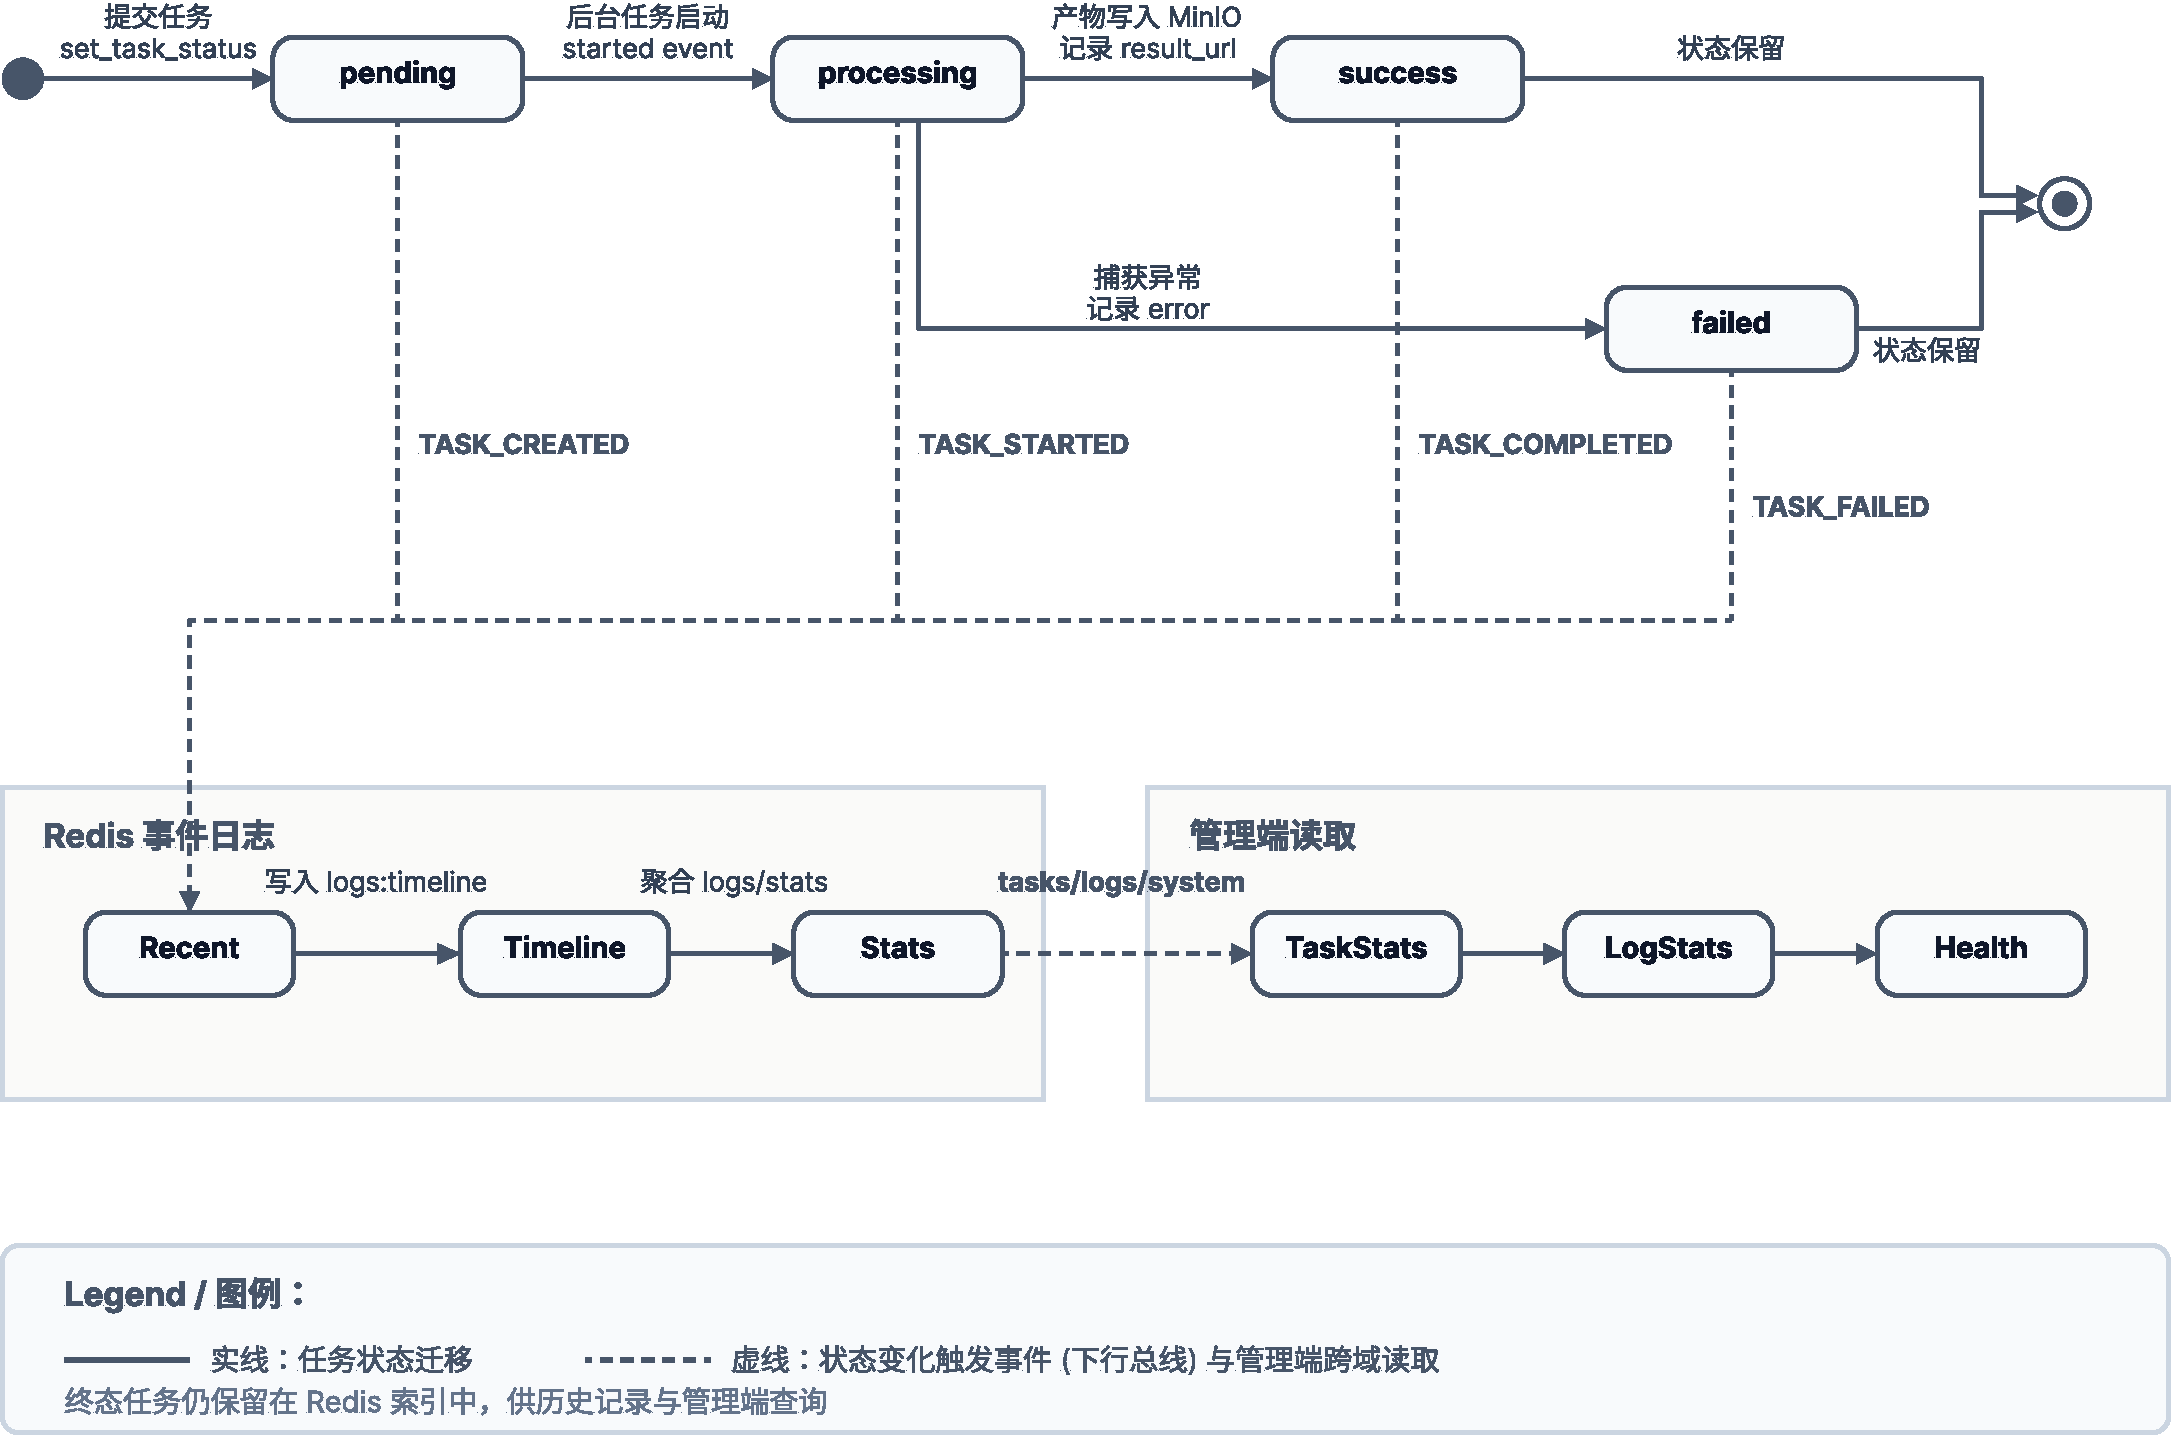
\includegraphics[width=0.92\textwidth,height=0.50\textheight,keepaspectratio]{figures-pdf/fig17-任务状态与事件流转图.pdf}
  \caption{任务状态与事件流转图}
  \label{fig:chap04-task-state-flow}
\end{figure}

\section{管理驾驶舱数据管线设计}

管理驾驶舱采用实时运行数据与历史分析样本并行的设计。实时运行数据直接来自 FastAPI 接口，适合反映当前文件数、任务数、失败数、队列长度、近期事件和服务健康；历史分析样本来自 Spark 输出，适合表达较长窗口下的文件类型分布、转换矩阵、趋势变化和质量分析。图 \ref{fig:chap04-analytics-pipeline} 展示了这一管线。该设计使用户端操作能够进入实时观察，同时保留大数据课程场景下的离线分析能力。

实时运行指标的计算以 Redis 中的任务集合与日志统计为基础。在式 \ref{eq:req-task-total} 的基础上，管理端第一屏的任务成功率与失败占比定义为：
\begin{equation}
  R_s=\frac{C}{\max(T,1)},\qquad
  R_f=\frac{F}{\max(T,1)}.
  \label{eq:task-rate}
\end{equation}
其中 $R_s$ 表示任务成功率，$R_f$ 表示失败占比，分母使用 $\max(T,1)$ 是为了避免任务总量为零时产生无意义除法。近 24 小时事件规模直接来自日志统计，记为 $L_{24}=E_{24}$。式 \ref{eq:task-rate} 对应前端读取的 \texttt{/api/v1/tasks/stats}、\texttt{/api/v1/tasks/queue-length} 与 \texttt{/api/v1/logs/stats}，用于解释管理端实时数值会随业务操作发生变化。

\begin{figure}[H]
  \centering
  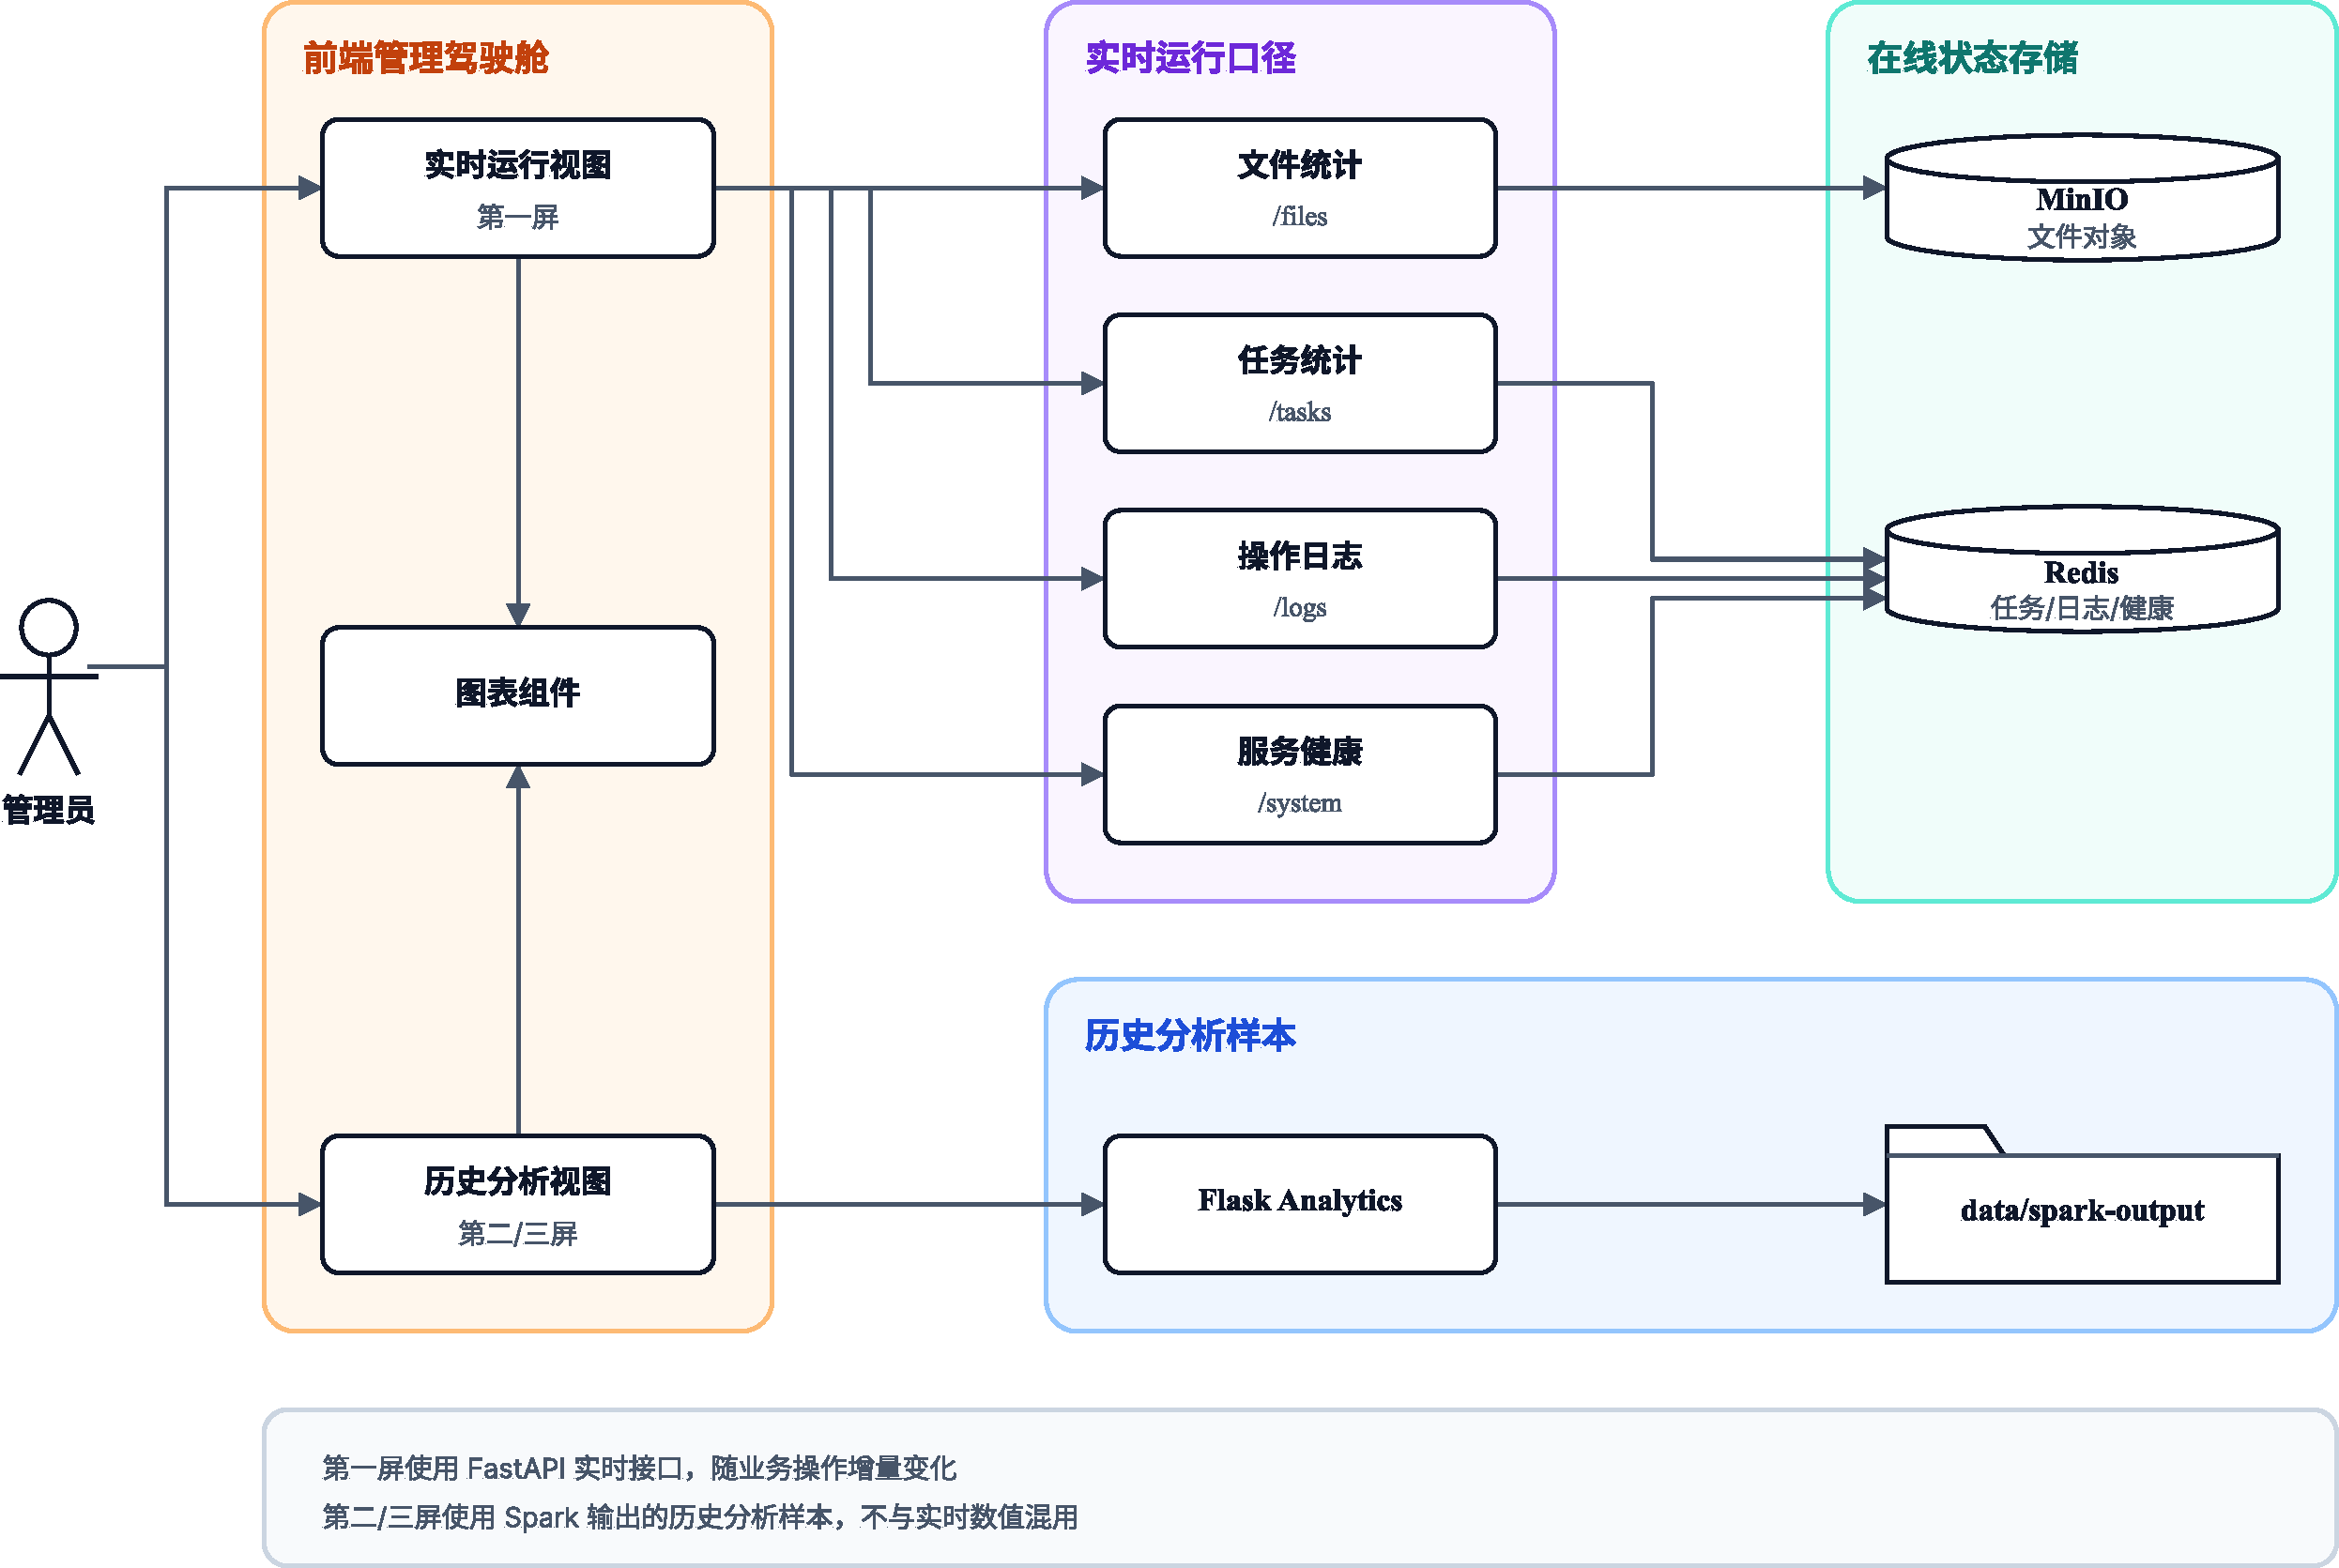
\includegraphics[width=0.96\textwidth,height=0.52\textheight,keepaspectratio]{figures-pdf/fig14-管理驾驶舱数据管线图.pdf}
  \caption{管理驾驶舱数据管线图}
  \label{fig:chap04-analytics-pipeline}
\end{figure}

\section{部署结构设计}

系统采用本地进程管理与容器化基础依赖结合的部署方式。前端开发服务与 Flask 分析服务适合使用 PM2 管理，便于快速重启、查看日志和保留长期运行状态；Redis、MinIO、Gotenberg 等基础依赖适合由 Docker Compose 管理，确保端口、网络和数据卷稳定。FastAPI 主服务启动时初始化 MinIO、Redis 和健康检查循环，保证 API 可用性与基础依赖状态能够被系统状态接口观察到。

从启动顺序看，Redis、MinIO 和 Gotenberg 属于基础依赖，应先于 FastAPI 主服务启动；FastAPI 启动后负责创建存储桶、注册路由和启动健康检查循环；前端与 Flask Analytics 则可以作为独立展示服务由 PM2 持续守护。这样的部署边界使文件处理主链路与历史分析展示链路可以单独重启，降低调试管理端图表时影响用户端上传和转换的概率。

从运行观测看，系统状态接口需要同时覆盖 API、对象存储、任务状态、转换服务和分析服务。若 MinIO 不可用，文件上传和下载会失败；若 Redis 不可用，任务状态和近期事件会失去持久记录；若 Gotenberg 不可用，Office 转 PDF 和部分预览链路会降级。将这些依赖纳入系统状态设计，可以让管理端显示的不只是页面是否打开，而是关键业务能力是否可用。

\section{本章小结}

本章完成了 CulCloud 的系统总体设计，明确了分层架构、模块边界、业务流程、数据结构、运行指标和部署结构。通过业务闭环、任务状态、数据模型和管理管线的组合设计，系统能够把用户端动作转换为可查询任务、可下载产物和可观察指标。

从总体架构看，系统采用前端界面、FastAPI 业务接口、领域服务、对象存储、运行状态和历史分析服务分层组织。该结构的好处是职责边界清晰：前端负责交互和状态展示，FastAPI 负责接口校验和业务编排，MinIO 负责文件对象保存，Redis 负责任务与日志状态，Gotenberg 负责重型文档转换，Spark 与 Flask Analytics 负责历史分析结果读取。不同模块之间通过 API 和对象键建立联系，而不是相互直接读取内部实现。

从业务流程看，本章把上传预览、格式转换、PDF 页面处理和管理端观察放入同一条闭环中分析。文件上传会形成对象和日志，文件预览会形成可复用缓存，转换和 PDF 导出会形成异步任务与结果产物，管理端再读取这些状态形成运行指标。这样的设计使系统不只是多个页面的集合，而是一个可追踪、可解释、可复现的资料处理平台。

从数据和运行角度看，系统没有引入复杂关系数据库，而是利用对象名前缀、任务状态集合和事件日志完成当前阶段所需的数据表达。该选择降低了本地部署和验证成本，但也要求在对象移动、目录删除、预览缓存和转换产物之间保持清晰边界。后续若引入用户权限、共享协作和长期审计，可以在现有对象键和任务标识基础上补充关系索引。

从设计边界看，本章确认的是最小可用平台的总体结构，而不是完整企业级云盘方案。当前设计重点覆盖单用户资料管理、轻量文件处理、异步任务可追踪和管理端观察；对于细粒度权限、多人协同编辑、跨设备同步冲突、对象版本回滚和长期归档策略，只保留可扩展位置。这样能够让系统在课程实践规模内保持可运行、可说明，同时为后续增强留下清晰方向。

因此，第 4 章承担的是“把系统如何组织起来”讲清楚的任务，而不是替代后续实现说明。

下一章将在本章设计基础上进一步落到代码实现，说明各前端视图、API 客户端、后端路由、领域服务和数据对象之间如何协作；第 6 章则从功能用例、命令行结果和业务闭环三个层面验证这些设计是否真正落地。
